\documentclass[a4paper,12pt]{article}
\usepackage[utf8]{inputenc}
\usepackage{amssymb,amsmath,uniinput,graphicx,hyperref, multirow,siunitx}
\usepackage[section]{placeins}
\usepackage[ngerman]{babel}
\usepackage[left=3cm,right=3cm,top=3cm,bottom=3cm]{geometry}
\renewcommand{\familydefault}{\sfdefault}
\setlength{\belowcaptionskip}{6pt}
\hypersetup{pdfinfo = {
	Title={Versuchsprotokoll zu Positronen im Festkörper},
	Author={Knut Kiesel, Tobias Pook},
	Keywords={Teilchenfalle}
}}


\graphicspath{ {../pictures/} }
\title{Laborpraktikum Teilchenphysik\\ Lebensdauer von Positronen im Festkörper}
\author{Knut Kiesel\\Tobias Pook}
\date{\today}

\begin{document}
\maketitle
\vspace{5cm}
\tableofcontents
\thispagestyle{empty}
\newpage
\setcounter{page}{1}

\section{Ziel des Versuches}
Ziel des Versuches ist der Aufbau und die Inbetriebnahme einer Messstation,
die in der Lage ist die Lebensdauer von Positronen in Festkörpern in der
Größenordnung von $\SI{100}{ps}$ zu messen.

Da die Annihilationswahrscheinlichkeit von der Energie abhängig ist,
müssen die Positronen thermalisiert werden.
Dies dauert bei Aluminium wenige $\si{ps}$.
In Isolatoren oder amorphen Stoffen dauert die Abbremszeit sehr viel länger,
sodass sich das Positron mit einem Elektron des Festkörpers zu einem Positronium verbinden können,
wenn die Affinitäten von Elektron und Positron kleiner
als die Affinität von Positronium und dessen Bindungsenergie ist.
Hier gibt es zwei Möglichkeiten: Parapositronium mit entgegengesetztem Spin und Orthopositronium mit gleichgerichtetem Spin.
Orthopositronium hat eine längere Lebensdauer, weil es nur in drei Photonen zerfallen kann, was unwahrscheinlicher als der Zerfall in zwei Photonen ist.
Durch Elektronenaustausch wandelt es sich oft in Parapositronium um, welches durch den Zerfall in zwei Photonen eine kürzere Lebenszeit hat.

Als Positronenquelle wird in diesem Versuch $^{22}$Na verwendet, welches beim Zerfall in $^{22}$Ne
zuerst ein γ-Quant der Energie $\SI{1.28}{MeV}$ abgibt und dann ein Positron emittiert.
Nach einer vom Festkörper abhängigen Zeit annihiliert das Positron unter Aussendung
von zwei bis drei γ-Quanten mit einer Energie von $\SI{511}{keV}$.
Durch das messen der Zeitdifferenz zwischen dem ersten γ-Quant des Übergangs und dem
γ aus der Annihilation kann die Lebensdauer des Positrons bestimmt werden.


\section{Aufbau und Durchführung}
%Kommentare aus der Vorbesprechung:
%	Constant Fraction Discriminator liefert logisches out bei BLD Ausgang
%	Die Delay Einheit ändert die polarität des Signal, wenn gewünscht.
%	Der Multi Channel Analyzer nimmt nur positive Signal ohne Offset an.

Der Detektor, zu sehen in Abbildung \ref{fig:quelle},  besteht aus zwei zylindrischen Szintiallatonsdetektoren,
 welche in einem Gehäuse mit einem Photomultiplier verbaut sind.
\begin{figure}[htb]
		\centering
		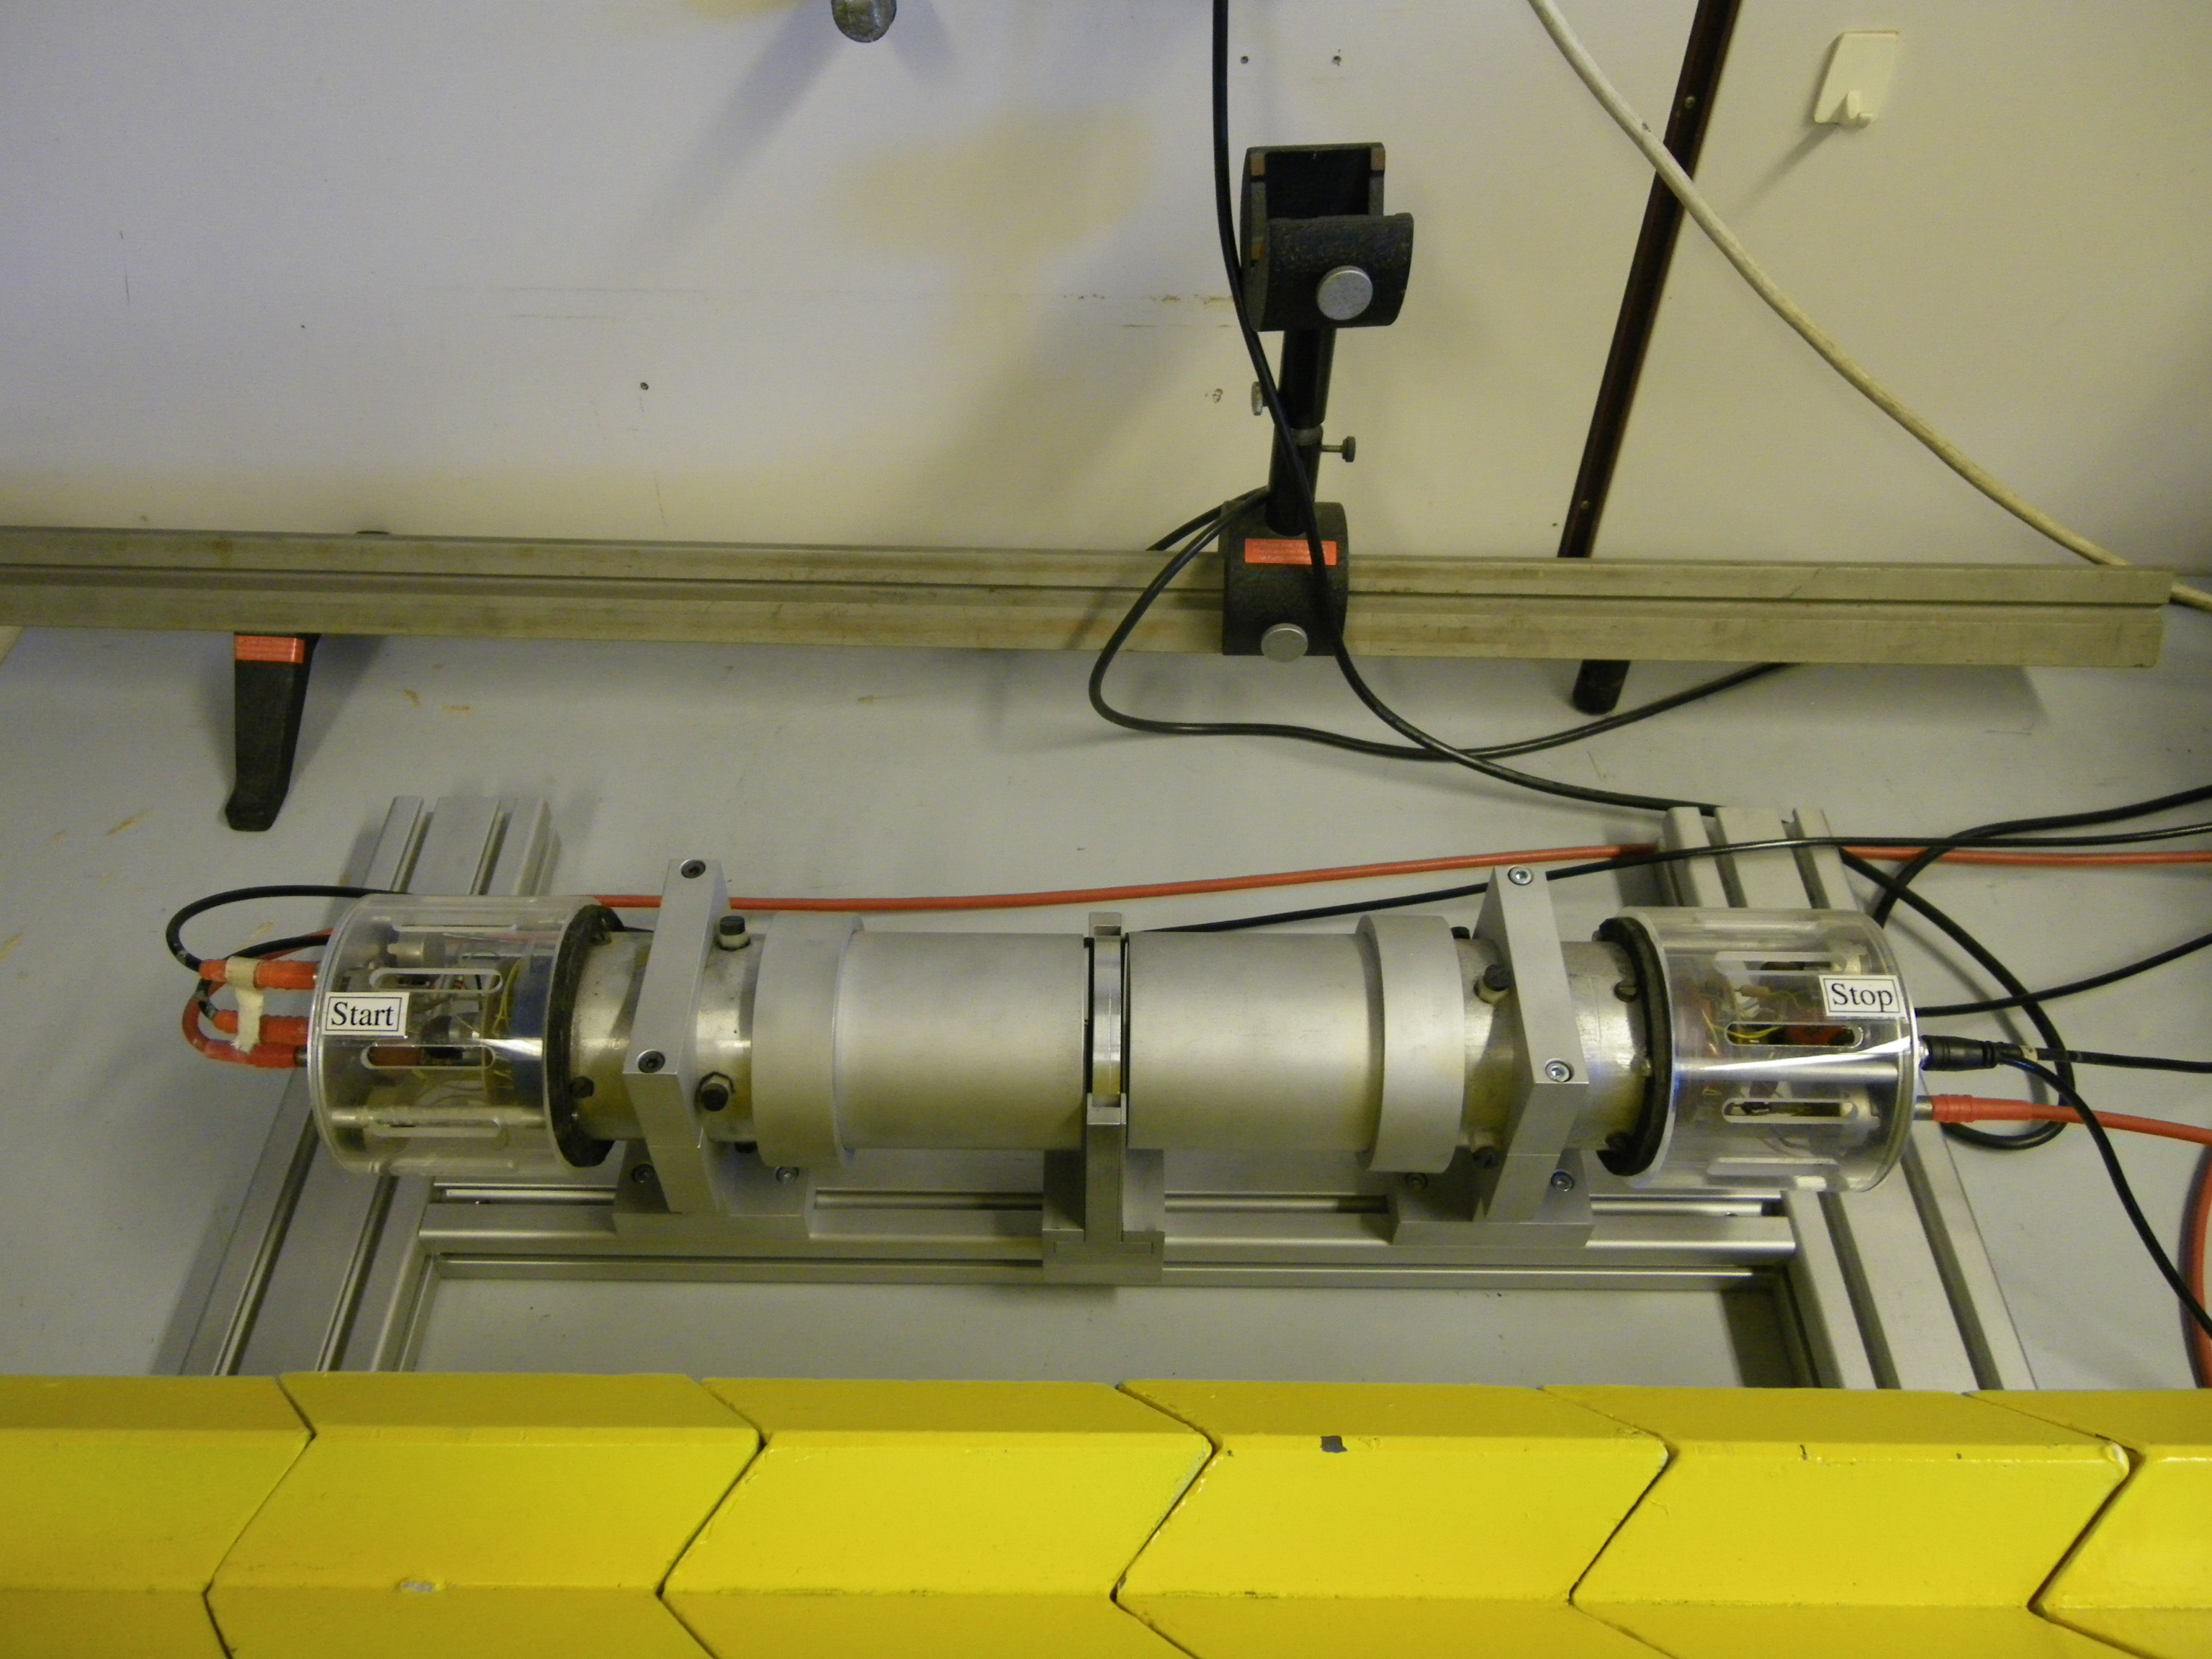
\includegraphics[width=0.5\textwidth]{quelle2.jpg}
		\caption{Scintilatoren mit Photomultiplier und Quelle}
		\label{fig:quelle}
\end{figure}

Die radioaktiven Proben werden zwischen beiden Szintillatoren platziert.
An der Katode des Photomultipliers wird  eine Spannung von von $\SI{-2}{kV}$ angelegt.
Damit sind die Anodensignale noch nicht Übersättigt.
Von beiden Photomultipliern wird sowohl das Anodensignal als auch das Dynodensignal, also das Signal an der letzten Dynode, abgegriffen.
Das Dynodensignal ist ein leicht positives Signal, dessen Pulse aus stark schwankenden kleineren Pulsen besteht, trotzdem aber eine Höhe hat, die Energie abhängig ist.
Das Signal wird für die Energiemessung und damit für das Gate verwendet.

Das Anodensignal ist ein Puls mit negativem Ausschlag und eine der Energie entsprechenden Höhe.
Es wird für das Messen der Zeitabstände benutzt, da das Dynodensignal mit den starken Schwankungen genaue schnelle Messungen von kleinen Zeitabständen nicht zulässt.

Es liefert für das Dynoden- und das Anodensignal jeweils ein Photomultiplier das Start und der andere das Stoppsignal.

Durch die Trennung in Anodensignal und Dynodensignal kann man den Schaltkreis in zwei unabhängige Kreise unterteilen, die nur an einer Stelle wieder zusammenlaufen.
Sie werden "`schneller"' und "`langsamer"' Kreis genannt.

Der Aufbau ist in Abbildung \ref{fig:aufbau} zu sehen.
\begin{figure}[htb]
		\centering
		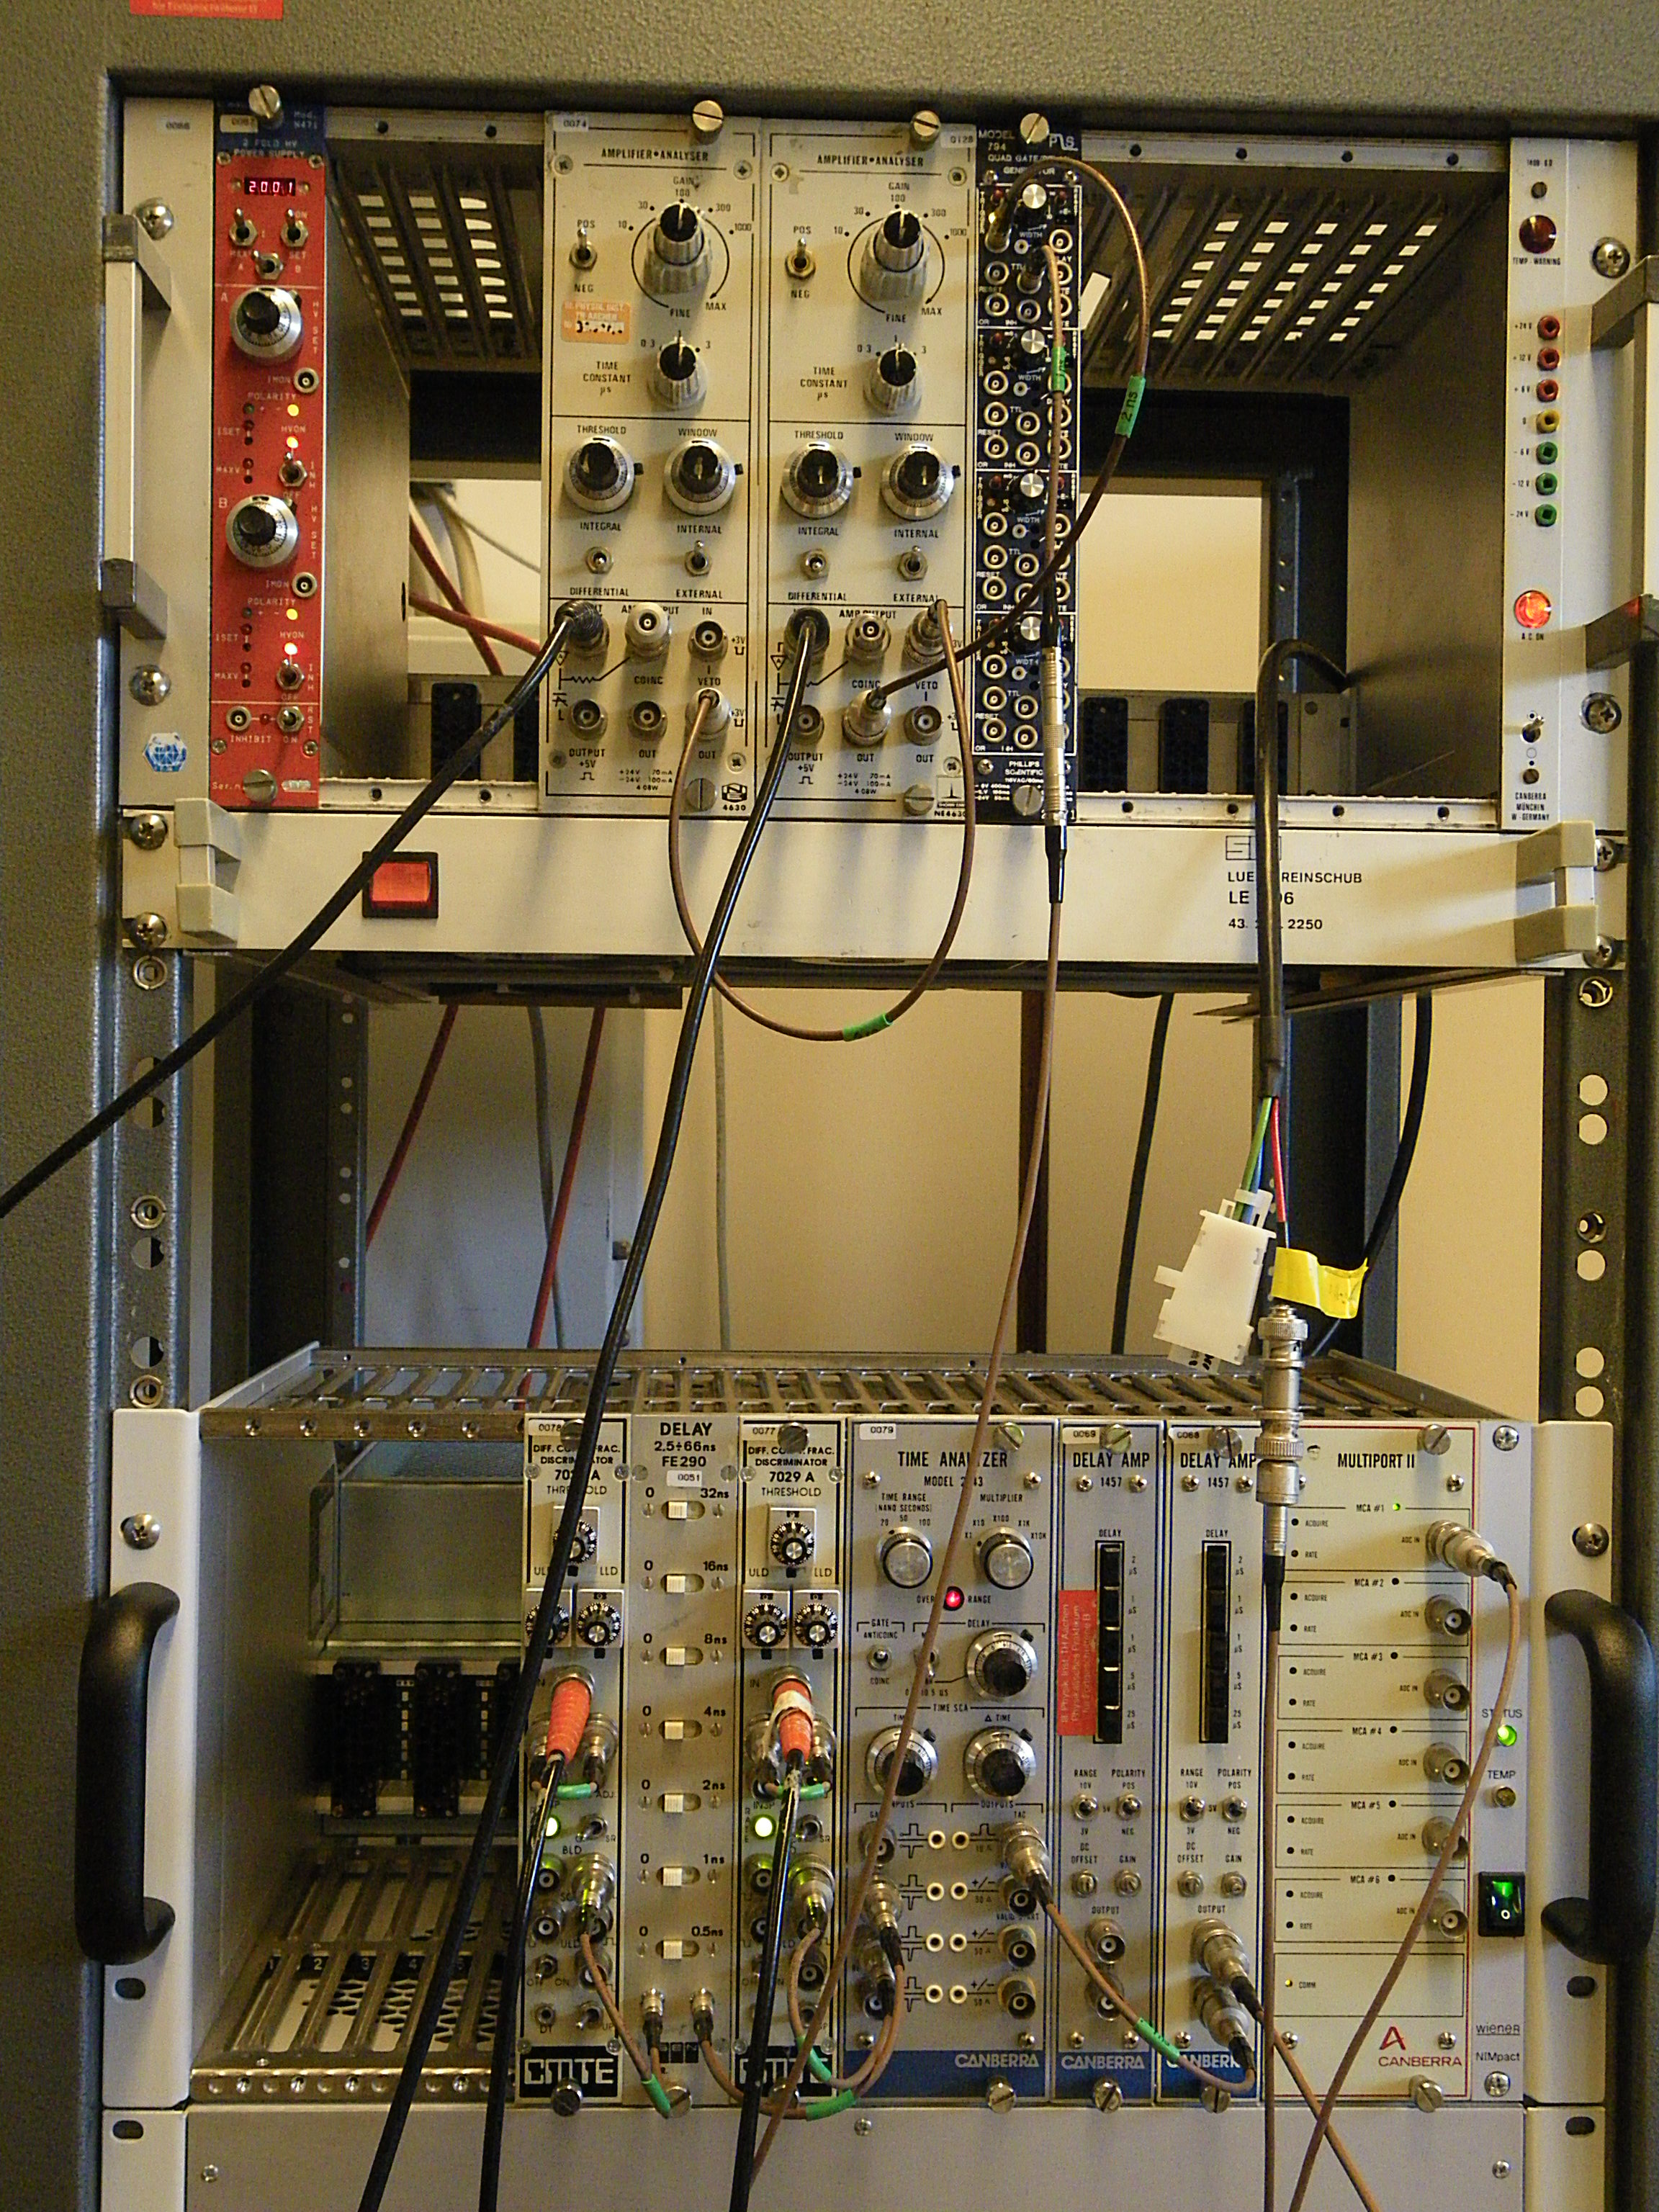
\includegraphics[width=.5\textwidth]{aufbau.jpg}
		\caption{Photo der elektronischen Verschaltung}
		\label{fig:aufbau}
\end{figure}

Links oben befindet sich die rote Spannungsquelle, daneben zwei Amplifier Analyzer mit Koinzidenzstufe\footnote{Nuclear Enterprises, Modell 4630} für Start und Stopsignal des langsamen Kreises.
Als letztes in der oberen Reihe ist das ein Quad Gate\footnote{Fa. Phillips Scientific, Modell 794} zu sehen.

In der unteren Reihe umgeben zwei Differential Constant Fraction Discriminatoren\footnote{Fa. Stanford Research Systems Inc., Modell DG535} eine Delay Einheit\footnote{Fa. SEN, Modell FE290}.
Rechts daneben befindet sich ein Time Analyser\footnote{Fa. Canberra, Modell 2043}, zwei Delaystufen\footnote{DFa. Canberra, Modell 1457} und zuletzt ein Vielkanalanalysator\footnote{Multiport II, Fa. Canberra} der auf der Rückseite mit einem Computer und dem Gate verbunden ist.

Schematisch ist der Aufbau in Abbildung \ref{fig:schaltplan} zu sehen.
\begin{figure}[htb]
		\centering
		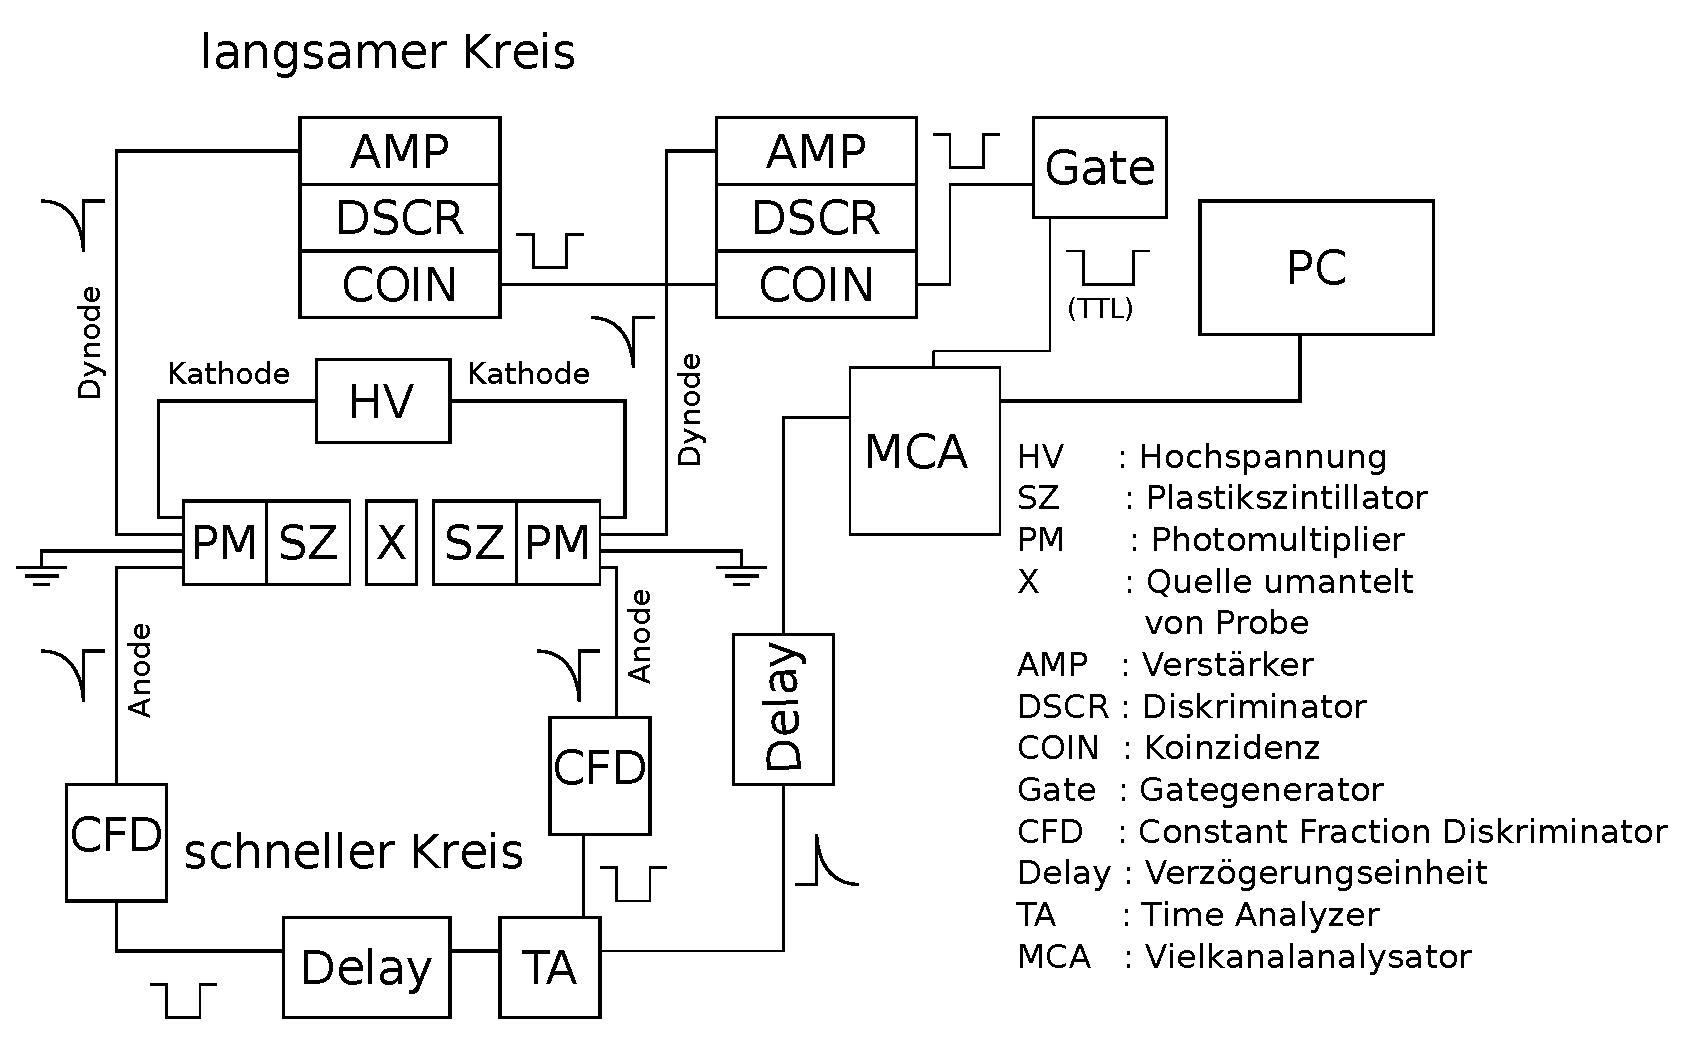
\includegraphics[width=1.0\textwidth]{Schaltplan_custom.pdf}
		\caption{Schematischer Schaltplan des Aufbaus des Versuchs.
		An den Seiten sind die Signalformen (logisch/analog) angegeben.}
		\label{fig:schaltplan}
\end{figure}

Wie schon oben genannt und wie auch in der Abbildung zu sehen, wird der Schaltkreis in zwei Kreise unterteilt:
\begin{itemize}
	\item
	Der langsame Kreis prüft ob sich die gemessenen Photonen sich im richtigen Energieintervall 
	befinden und erzeugt abhängig davon ein Triggersignal, das das Gate des Vielkanalanalysators öffnet.
	\item
		Der schnelle Kreis bestimmt die Zeitdifferenz und gibt dieses in Form eines Pulses an den
	Vielkananlanalysator weiter.
\end{itemize}
\subsection*{Langsamer Kreis}
Für den langsamen Kreis wird das Dynodensignal der Photomultiplier genutzt und in jeweils einem
Einzelkanaldiskriminator (\textbf{EKD}) weiter verarbeitet.
Dieser verstärkt das Signal zunächst (es wird ein Gain von 300 eingestellt),
damit sich das Energiespektrum im Vielkanalanalysator über möglichst alle Kanäle erstreckt.
% Erklären was beim Differenzieren passiert.
Das Dynodensignal besitzt eine ausreichende Abhängigkeit zwischen Energie und Pulshöhe
um ein (nicht kalibriertes) Energiespektrum mit Hilfe des Vielkanalanalysator aufzuzeichnen.

Anschließend werden die Schwellwerte des Diskriminators im EKD so eingestellt,
dass nur Teilchen mit einer höheren Energie als die rechten Flanke des Anhilationspeak als
Startsignal (Fenster 2 in Abbildung \ref{fig:auswahl}) genutzt werden
und Teilchen in einem niedrigeren Energiefenster als Stoppsignal.

Wenn ein Teilchen im richtigen Energiefester ist, wird an einem Ausgang ein logisches Signal erzeugt,
was über das Gate zusammen mit dem verstärkten Dynodensignal in den Vielkanalanalysator geleitet wird.

Um eine Ober-und Untergrenze zu setzen, muss das Signal zuvor Differenziert werden,
was auch mit diesem Gerät möglich ist\cite{linearAmplifier}.

Das Stopsignal soll bei einer Annihilation eines Positrons entstehen
und deshalb eine Energie von $\SI{511}{keV}$ haben.
In Abbildung \ref{fig:auswahl} ist dies Fenster 1.
Zusätzlich wird eine untere Grenze bei 260±10
eingestellt um den Untergrund durch niederenergetischer Teilchen und elektronisches Rauschen des Photomultipliers zu reduzieren.
Die obere Grenze bei Kanal 3640±30 ist gleichzeitig die Grenze für das Startsignal,
bei dem ein $\SI{1.28}{MeV}$ Photon erwartet wird.
Diese Grenze ist sehr viel ungenauer,
da das Setzen des Schwellenwerts nicht für einen steilen Abbruch des Spektrums sorgt, sondern nur für ein weiches Abfallen.

% erkläre veto-out und veto-in, was genau machen die, und warum fuktioniert das?
Nachdem die Fenster für Start und Stoppsignal zunächst mit dem verstärkten Dynodensignal eingestellt sind,
wird der logische 'Veto-Out' Ausgang des Start-EKD in den 'Veto-In' Eingang des Stop-EKD gesteckt und das logische Ausgangssignal über das Gate
in den Vielkanalanalysator gegeben.
Die EKD dienen damit auch gleichzeitig als Koinsidenzstufen.

\begin{figure}
	\centering
	\includegraphics[width=0.8\textwidth]{../analyse/auswahl.pdf}
	\caption{Das Energiespektrum von $^{22}$Na aus dem verstärktem und vorgeglätteten
		Dynodensignal.
		Man sieht von rechts nach links bei Kanal 10000 den Peak des $\SI{1.28}{MeV}$ Photons,
		danach das Comptonkontinuum und bei etwa Kanal 3500 den Annihilationspeak.
		Am linken Rand (Kanal kleiner als 260) sieht man Rauschen, das ignoriert wird.
		Für ein Startsignal (Fenster 2) muss das ein größerer Kanal als 3630±100 angesprochen werden, 
		für ein Stopsignal ( Fenster 1) reicht ein Kanal größer als 260±10.}
	\label{fig:auswahl}
\end{figure}


\subsection*{Schneller Kreis}
Für den schnellen Kreis wird das Anodensigal der Photomultiplier genutzt.
Start und Stoppsignal werden zunächst in jeweils einem Constant
Fraction Discriminator (\textbf{CFD}) weiter verarbeitet.
Dieser erzeugt durch differenzieren zunächst einen bipolaren Puls aus dessen Nulldurchgang ein von der Pulsform unabhängiges Zeitsignal erzeugt wird
und in Form eines logischen Signal ausgegeben wird, wenn eine gewisse Pulshöhenschwelle überschritten wurde.
Um hier die Schwellen zu setzen, wird das logische Signal jeweils eines CFD über das Gate an den Vielkanalanalysator gesendet.
Die eigentliche Energieinformation bekommt man aus der Anode.
Ein Startsignal wird genauso definiert wie beim langsamen Kreis, das Stopsignal wird nur durch eine untere Schranke festgelegt (also Fenster 1 und 2 in Abbildung \ref{fig:auswahl}).
Als Schwellen werden am Gerät schließlich 9.0 bzw \dots eingestellt.

Nachdem die Schwellen gesetzt werden, kann das Startsignal in den Starteingang des Timeanalysers, das Stopsignal über ein schnelles Delay, das im Messzustand auf 0 gestellt ist, in den Stopeingang des Timeanalysers.
Der Time Analyzer erzeugt einen Puls, dessen Pulshöhe vom zeitlichen Abstand von Start und Stoppsignal ist.

Im Vielkanalanalysator werden die Pulse in ein Pulshöhenspektrum umgesetzt.
Um den schnellen und langsamen Kreis zeitlich aufeinander 
anzupassen ist zusätzlich eine Verzögerungseinheit zwischen Time Analyzer und den Vielkanalanalyser geschaltet, dessen Zeit auf $\SI{3}{μs}$ gestellt wird.

\section{Ergebnisse}
\subsection{Zeitkalibration}
Um die einzelnen Kanäle des VKA mit den entsprechenden Zeitabständen zu verknüpfen wird eine Zeitkalibration durchgeführt. Dazu werden
mit einem Pulsgenerator Pulse mit einer Amplitude von $3\si{V}$ und einer Pulsbreite von 10ns mit einer Frequenz von $1600\si{Hz}$ erzeugt.
Es wurde mit einem Oszilloskop sichergestellt, dass Form und Amplitude des erzeugten Puls denen aus dem Anodenausgang der Photomultiplier 
entsprechen. Das vom Pulsgenerator ausgegebene Signal wird durch ein T-Stück geteilt. Eine Abzweigung des T-Stück wird in den für das Startsignal vorgesehene 
CFD geleitet, die andere in eine Delayeinheit und dann in den CFD für das Stoppsignal. Vor der eigentlichen Kalibrierung wird das Delay getestet, indem
das Signal vor und nach dem Delay nicht durch die Constant Fraction Diskriminatoren sondern durch ein Oszilloskop abgegriffen werden. Hier lässt sich erkennen,
dass beide Signale bei ausschalten des Delay nahezu zeitgleich ankommen und in ihrer Pulsform erhalten bleiben. Es kann also ausgeschlossen werden das es zu 
zusätzlichen Verzögerungen oder sonstige Verfälschungen des Signal durch das T-Stück und die genutzten Kabel kommt.
Nach dem testen des Delay wird die ursprüngliche Verschaltung wieder hergestellt und die zeitlichen Abstände der logischen Signale der CFDs im Time Analyzer
in Pulshöhen umgesetzt. Die Pulse des Time Analyzer werden an den MCA weiter geleitet, dieser wird während der Kalibrierung mit
durchgehend geöffnetem Gate betrieben. Die Verzögerung wird am Delay in $0.5\si{ns}$ Schritten von $0\si{ns}$ bis $12\si{ns}$ erhöht, das aufgezeichnete Pulshöhenspektrum 
ist in Abbildung \ref{fig:timepuls} dargestellt. Es wird an jeden Peak im Spektrum eine Gaußfunktion angepasst, im folgenden werden die ausgewählten Zeitpunkte mit
dem Erwartungswert $\mu$ der angepassten Verteilung assoziiert und der Fehler auf diesen Wert als Breite des Peak $\sigma$ angenommen. Da es keine Möglichkeit gab 
(z.B. durch Vergleich mit einem weiteren Delay) die Unsicherheit auf die genutzten Verzögerungen zu bestimmen und es auch keine Angaben zu
den Unsicherheiten in der Betriebsanweisung des Bauteil zu finden waren wurde der Fehler auf die Verzögerung zu $0.075\si{ns}$ abgeschätzt also 
15\% der Verzögerungsschrittweite von $0.5\si{ns}$. An die so gewonnenen Zeit-Kanal Wertepaare wird eine Funktion angepasst, mit der im folgenden 
Kanalnummern in Zeitabstände umgerechnet werden. 

\begin{figure}
	\includegraphics[width=\textwidth]{../analyse/peaksToArray.pdf}
	\caption{Pulshöhenspektrum zur Zeitkalibration. Die Pulse haben einen Abstand von $0.5\si{ns}$}
	\label{fig:timepuls}
\end{figure}

\begin{figure}
	\includegraphics[width=\textwidth]{../analyse/singlePeak.pdf}
	\caption{Ein einzelner gaußförmiger Puls des Pulshöhenspektrum zur Zeitkalibration.}
	\label{fig:timesinglepuls}
\end{figure}
\subsection{Zeitnullpunkt und Zeitstabilität}
		\begin{figure}
		\includegraphics[width=0.8\textwidth]{../analyse/compareCo.pdf}
		\caption{Gemessenes Pulshöhenspektrum für $^{60}$Co vor und nach den $^{22}$Na Messungen}
		\label{fig:timepuls}
		\end{figure}
		Zur Bestimmung des Zeitnullpunkt und zum überprüfen der zeitlichen Stabilität werden Messungen mit $^{60}$Co durchgeführt, dieses Cobaltisotop liefert 
		beim Kaskadenzerfall in $^{60}$Co zwei zeitgleiche γ-Quanten mit Energien von $1,17\si{MeV}$ und $1,33\si{MeV}$. Es wird jeweils eine Messung vor Beginn
		und nach der Hauptmessreihen mit $^{22}$Na durchgeführt. Die Ergebnisse beider Messungen sind in Abbildung \ref{fig:compare_co} dargestellt.
		Da von einem Zeitgleichen eintreffen beider Pulse ausgegangen wird, dient die Position des beobachteten Peak im Pulshöhenspektrum als Zeitnullpunkt. Es
		ist zu erkennen das sich die Position des Peakmaximum während der Versuchdurchführung um 178 Kanäle verschoben hat. Diese Verschiebung entspricht einer
		Zeitdifferenz von lediglich xx ns. Die Änderung ist also im Rahmen der Messgenauigkeit klein genug um den Mittelwert der
		beiden gemessenen Peakpositionen , Kanal 4721 , als Nullpunkt für die Zeitmessungen zu benutzen. Die Veränderung des Nullpunkt wird im folgenden
		als zusätzlich systematische Unsicherheit auf alle Zeitmessungen angenommen. Die Zeitauflösung wird durch die mittlere Breite der beiden an die 
		Daten angepassten Gaußfunktion abgeschätzt.  
\subsection{Vergleich der Messungen für Aluminum und Polyethylen}
		
\subsection{Bestimmung der Lebensdauern in Polyethylen}
		
\subsection{Globaler Fit}
Die Fitfunktion für den globalen Fit, mal schau ob das noch was wird
\begin{align*}
	F(t) &= \frac{1}{2τ} \exp\left( \frac{2}{τ}\left( μ-t+\frac{σ^2}{τ} \right) \right) \frac{2}{\sqrt{π}}\int_{\frac{1}{\sqrt{2}σ}\left( μ-\frac{2σ^2}{τ} -t \right)}^\infty dγ e^{-γ^2}\\
	&= \frac{1}{2τ} \exp\left( \frac{2}{τ}\left( μ-t+\frac{σ^2}{τ} \right) \right) Erfc\left(\frac{1}{\sqrt{2}σ}\left( μ-\frac{2σ^2}{τ} -t \right)\right)
\end{align*}
\section{Diskussion}

 
\section{Diskussion} 
\end{document}
